\documentclass[10pt]{examdesign}
\usepackage{amsmath}
\usepackage{enumitem}
\usepackage{amsfonts}
\usepackage{pgfplots}
\usepackage{pifont}
\usepackage{graphicx}
\usepackage{fancyhdr}
\usepackage{cancel}
\usepackage{gensymb}
\usepackage[american]{circuitikz}

\SectionFont{\large\sffamily}
\Fullpages
\ContinuousNumbering
\usepackage{ulem}
\ProportionalBlanks{2}


\DefineAnswerWrapper{}{}
\NumberOfVersions{1}
%\IncludeFromFile{foobar.tex}
\examname{\Large{Semester 1 Review}}
\class {\Large AP Physics 1}

\def \namedata {Name: \hrulefill\\ 
	Date: \hrulefill \\
	Period: \hrulefill \\

			\begin{tabular}{| p{1cm} | p{1cm} | p{1 cm} | p{1cm} |}
	\hline
		+1 & 0 & -1 & $\Sigma$ 
		\\
		\hline
		& & & \vspace{.5cm}
		\\ \hline
	
	\end{tabular}
	\\
 \vspace{-.6in}
	
}




\begin{document}




\begin{multiplechoice} [title={Multiple Choice},
	rearrange=yes]


	
	\begin{question}
A blue sphere and a red sphere with the same diameter are released from rest at the top of a ramp. The red sphere takes a longer time to reach the bottom of the ramp. The spheres are then rolled off a horizontal table at the same time with the same speed and fall freely to the floor. Which sphere reaches the floor first?

	\end{question}

\begin{question}
An object is moving to the west at a constant speed. Three forces are exerted on the object. One force is 15 N directed due north, and another is 15 N directed due west. What is the magnitude and direction of the third force if the object is to continue moving to the west at a constant speed?



	\end{question}


\begin{question}
	An elevator carrying a person of mass m is moving upward and speeding up. How does the magnitude $F$ of the force exerted on the person by the elevator floor compare with the magnitude $mg$ of the gravitational force?

\end{question}


\begin{question}
A box with a weight of 50N is at rest on a horizontal surface. The coefficient of static friction between the box and the surface is 0.40, and the coefficient of kinetic friction is 0.20. A horizontal 20.0 N force is then exerted on the box. The magnitude of the acceleration of the box is most nearly - 


\end{question}

\begin{question}
	A diver initially moving horizontally with speed $v$ dives off the edge of a vertical cliff and lands in the water a distance $d$ from the base of the cliff. How far from the base of the cliff would the diver have landed if the diver  initially had been moving horizontally with speed $2v$?

\end{question}

\begin{question} An object is thrown with a horizontal velocity of 30 m/s from a cliff that is 225 m above level ground.  If air resistance is negligible, the time that the object takes to fall to the ground is most nearly - 

\end{question}


\begin{question}
A spacecraft is drifting through space at a constant velocity.  Suddenly, a gas leak in the side of the spacecraft gives it a constant acceleration in a direction perpendicular to the original velocity.  The orientation of the spacecraft does not change, so the acceleration remains perpendicular to the original direction of the velocity.  What is the shape of the path the spacecraft moves along?  

\end{question}

\begin{question}
	An athlete sitting in a wheelchair at rest throws a basketball forward. Since the athlete and the wheelchair have greater mass than the basketball has, the athlete and the wheelchair will — 

\end{question}


\begin{question}
	The Voyager 2 Spacecraft was launched on August 20 1977.  It flew past the planets Jupiter, Saturn, Uranus and Neptune.  Though it has no fuel left, it continues to fly away from the earth, and is currently twice as far from the sun as the dwarf planet Pluto.  If it is left alone, it will pass close to the star Sirius in the year 298,000.  Which of Newton's Laws best explains why Voyager 2 continues to travel farther from the earth?

\end{question}

\begin{question}
	Billy-Bob is showering in the locker room after a football game when he drops the soap.  The soap slides all the way across the locker room without a significant decrease in speed, and does not stop until it hits the wall.  This is because - 

\end{question}

\begin{question}
	Homer is 18 meters from Barney, who has just stolen Homer's keys.  Homer is running at a speed of 5 m/s and Barney is running at a speed of 3 m/s.  How long will it take Homer to catch up to Barney?

\end{question}


\begin{question}
	A person is running on a track. What force propels the runner forward? 

\end{question}

\begin{question}
	An astronaut is standing on the moon.  He holds a hammer in one hand and a feather in the other.  What happens when he lets them go, and why?

\end{question}


\begin{question}
	A rocket has an acceleration of 11 m/s\textsuperscript{2}.  If it accelerates at this rate for 10 minutes, what will its final speed be?

\end{question}

\begin{question}A stream is flowing to the north at 0.4 m/s.  A duck swims in the stream, and paddles directly to the east at 0.5 m/s. What is the resultant speed of the duck relative to a person standing on shore?  

\end{question}

\begin{question}
	Two tug of war teams pull on opposite ends of a rope:
	
	\begin{center}
			\includegraphics[height={.5in}]{tug.png}
	\end{center}

	
	 Each team exerts a horizontal force of 6000 N.  If the mass of the entire system is 400 kg, the acceleration of the system will be - 

\end{question}


\begin{question}
	
	A 2 kg block slides down an inclined plane, as shown in the picture below:  
	
	\begin{center}
		\includegraphics[height={0.75in}]{incp.png}
	\end{center}	
	
	
Draw a diagram that correctly represents \textbf{f}, the frictional force, \textbf{N}, the normal force, and \textbf{W}, the weight of the block?
	\vspace{1in}
	

\end{question}


\begin{question}
	Billy-Bob is riding his bike.  The combined mass of Billy-Bob and his bike is 100 kg.  Starting from a stop, he applies a force of 225N to the bike.  His bike accelerates at a rate of 1 m/s\textsuperscript{2}.  What is the frictional force acting on the bike? 

\end{question}



\begin{question}
	In a movie, a criminal is trying to escape from the police by driving at 50 m/s. The police are driving at a speed of 60 m/s.  If the criminal is 500 m from the police, how long will it take the police to catch up to the criminal?  

\end{question}



\begin{question}
	A marble rolls off the top of a flat, level roof with an initial velocity of 3.5 m/s.  If the height of the building is 10 meters, what is the horizontal component of the marble's velocity when it hits the ground?

\end{question}


\begin{question}
	 A man in a blue canoe and a woman in a pink canoe are racing.  Both canoes start from rest, but accelerate at different constant rates, $a_{pink}$ and $a_{blue}$, respectively.  The pink canoe travels 1.4 times farther than the blue canoe in the same amount of time. What is the relationship between the acceleration of the pink canoe and the acceleration of the blue canoe?

\end{question}



\begin{question}
	A ball rolls off a cliff with an initial velocity of 13 m/s.  It lands 14.5 meters away.  How tall was the cliff?

\end{question}

\begin{question}
Sara throws the same ball four times.  The trajectories are shown below. Assuming that air resistance is negligible, which ball stayed in the air the shortest amount of time? 

\includegraphics[height={1in}]{proj.png}


\end{question}



\begin{question}
	A 75 kg astronaut pushes on a 2000 kg satellite, causing the satellite to move with an acceleration of 0.2 m/s\textsuperscript{2}. According to Newton's Third Law, what is the astronaut's acceleration?

\end{question}


\begin{question}
	Two bicycle riders, Lance and Floyd, are racing each other. Lance has a greater top speed of 25 m/s, compared to Floyd's 20 m/s.  However, Floyd has a greater acceleration of 3 m/s\textsuperscript{2}, compared to Lance's 2 m/s\textsuperscript{2}.  Which of the riders will win the race?

\end{question}




\begin{question}
	On a newly discovered planet, a ball is dropped from a cliff of unknown height, $h_1$.  It takes the ball exactly 1 second to reach the ground.  The same ball is dropped from a second cliff of height $h_2$, where it takes the ball 5 seconds to hit the ground.  What is the relationship between the heights of the two cliffs?  

\end{question}

\begin{question}
	A train is traveling to the right with a constant speed $v_t$.  Two identical spheres are rolling on the floor of one train car.  In the frame of reference of the train, the spheres are moving directly toward each other with a speed $v_p$, parallel to the train's motion, as shown in the figure above.  A person is standing outside the train as it passes by.  What are the velocities that the person would measure of each of the spheres as the train passes by? 
	
	\begin{center}
		\includegraphics[height=0.5in]{train2.png}  
	\end{center}
	
	

	
\end{question}

\begin{question}
	A student standing on the roof of a 60-meter tall buliding kicks a stone with an initial horizontal speed of 4 m/s, as shown in the diagram.  How much time is required for the stone to reach the ground below? 

 \hspace{2 in} \includegraphics[height=1.1in]{building.png}
	
\end{question}


\begin{block}
	\textit{	The following two questions refer to the following information:}
	
	\includegraphics[height=0.5in]{bball.png} 
	
	During a drill in basketball practice, a player runs the length of a 30 meter court and back.  The player does this four times in 60 seconds. 
	
	\begin{question}
		What is the magnitude of the player's displacement at the end of the drill? (Hint: Magnitude means number only and not direction.)
	
	\end{question}
	
	
	\begin{question}
		What is the player's average speed during this drill? 

	\end{question}
\end{block}

\begin{question}
	An airplane is traveling north at 240 m/s when it encounters a 60 m/s crosswind from west to east.  What is the resultant speed of the plane, rounded to the nearest whole number? 

\end{question}



\begin{question}
	On Earth, what is the force of gravity, in newtons, on a 13 kg object?

	
\end{question}





\begin{question}
	Blocks of brass with various masses are dragged across a table.  The frictional force and normal force for each block are shown below: 
	
	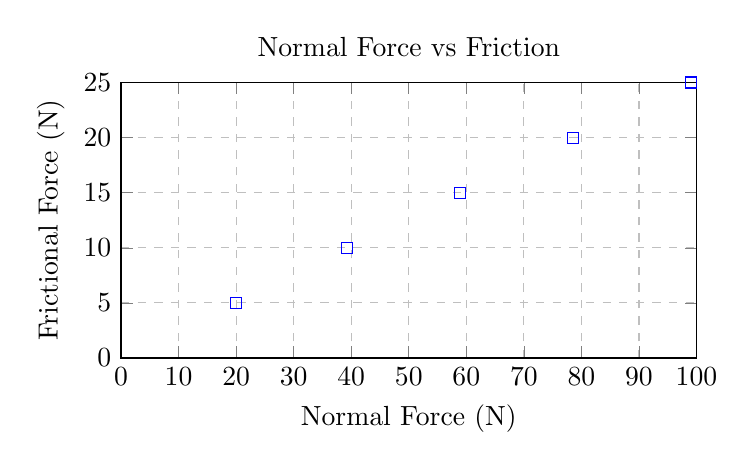
\begin{tikzpicture}
	\begin{axis}[only marks,
	title={Normal Force vs Friction},
	xlabel={Normal Force (N)},
	ylabel={Frictional Force (N)},
	xmin=0, xmax=100,
	ymin=0, ymax=25,
	xtick={0,10,20,30,40,50,60,70,80,90,100},
	ytick={0,5,10,15,20,25},
	ymajorgrids=true,
	xmajorgrids=true,
	grid style=dashed,
	legend pos=south east,
	height=2in,
	width=3.5in
	]
	
	\addplot[
	color=blue,
	mark=square,
	]
	coordinates {
		(20,5)(39.24,10)(58.86,15)(78.48,20)(99,25)};
	
	
	
	
	
	\end{axis}
	\end{tikzpicture}
	
	What is the best estimate of the coefficient of kinetic friction between brass and the table?

\end{question}






\end{multiplechoice} 
\pagebreak

	


\end{document}


